\chapter{Implementación, Pruebas y Resultados}
\label{chap:implementacion}

\section{Descripción de la Solución}
\textit{[Presentar detalladamente la solución implementada, indicando los componentes desarrollados, configurados o integrados.]}

\section{Proceso de Implementación}
\textit{[Describir paso a paso la ejecución técnica del proyecto, incluyendo desarrollo o configuración, integración de componentes y despliegue en un entorno real o controlado.]}

\section{Pruebas y Validación}
\textit{[Describir las pruebas realizadas para validar el funcionamiento de la solución, tales como pruebas funcionales, integrales, de seguridad, rendimiento o conectividad, según aplique.]}

\section{Resultados}
\textit{[Presentar los resultados obtenidos durante la validación, comparando la situación inicial con la posterior a la implementación. Incluir métricas, indicadores o evidencias.]}

\subsection{Ejemplo de Figura 2}
Como ejemplo de mención con referencia: en la Figura~\ref{fig:ejemplo_2} se observa una salida visual que puede emplearse para documentar arquitectura o resultados.

\begin{figure}[htbp]
  \centering
  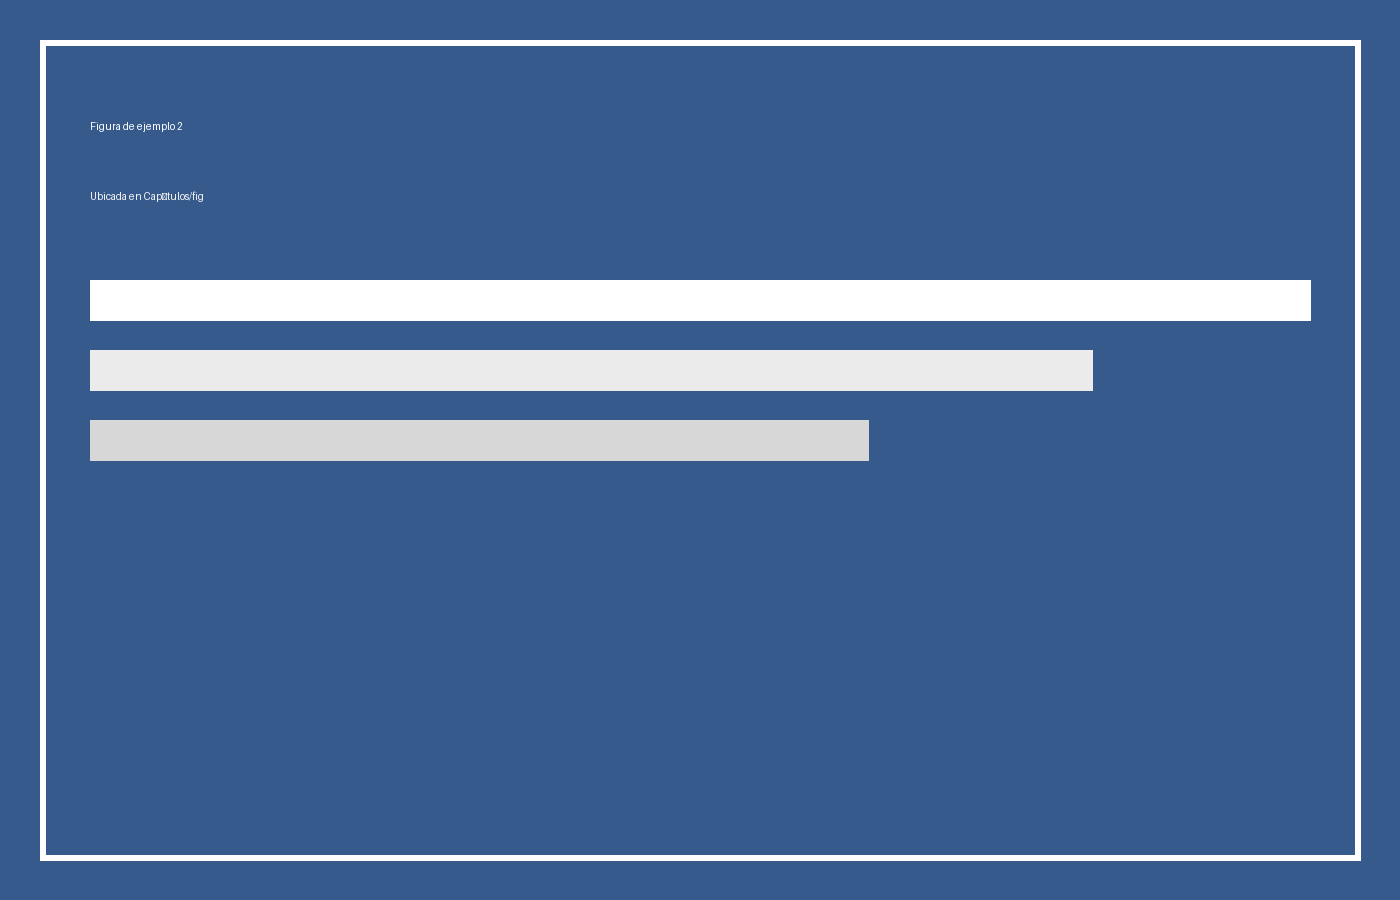
\includegraphics[width=0.80\textwidth]{Capítulos/fig/fig_ejemplo_2.png}
  \caption{Ejemplo de figura para presentar resultados o arquitectura implementada.}
  \label{fig:ejemplo_2}
\end{figure}
\elaboradopor{Estudiante}
\fuente{Elaboración propia}

\subsection{Ejemplo de Tabla 2}
Como ejemplo de mención con referencia: la Tabla~\ref{tab:ejemplo_2} muestra una comparación antes/después para análisis cuantitativo.

\begin{table}[htbp]
  \centering
  \caption{Ejemplo de tabla comparativa antes y después de la implementación.}
  \label{tab:ejemplo_2}
  \begin{tabular}{|l|c|c|}
    \hline
    Métrica & Antes & Después \\
    \hline
    Tiempo de respuesta (ms) & 850 & 320 \\
    \hline
    Disponibilidad (\%) & 96.2 & 99.3 \\
    \hline
    Tasa de error (\%) & 4.8 & 1.2 \\
    \hline
  \end{tabular}
\end{table}
\elaboradopor{Estudiante}
\fuente{Resultados de pruebas funcionales}

\subsection{Ejemplo de Imagen 2}
Como ejemplo de referencia narrativa: la Imagen~\ref{img:ejemplo_2} permite incorporar evidencias de interfaz o panel operativo.

\begin{imagen}[htbp]
  \centering
  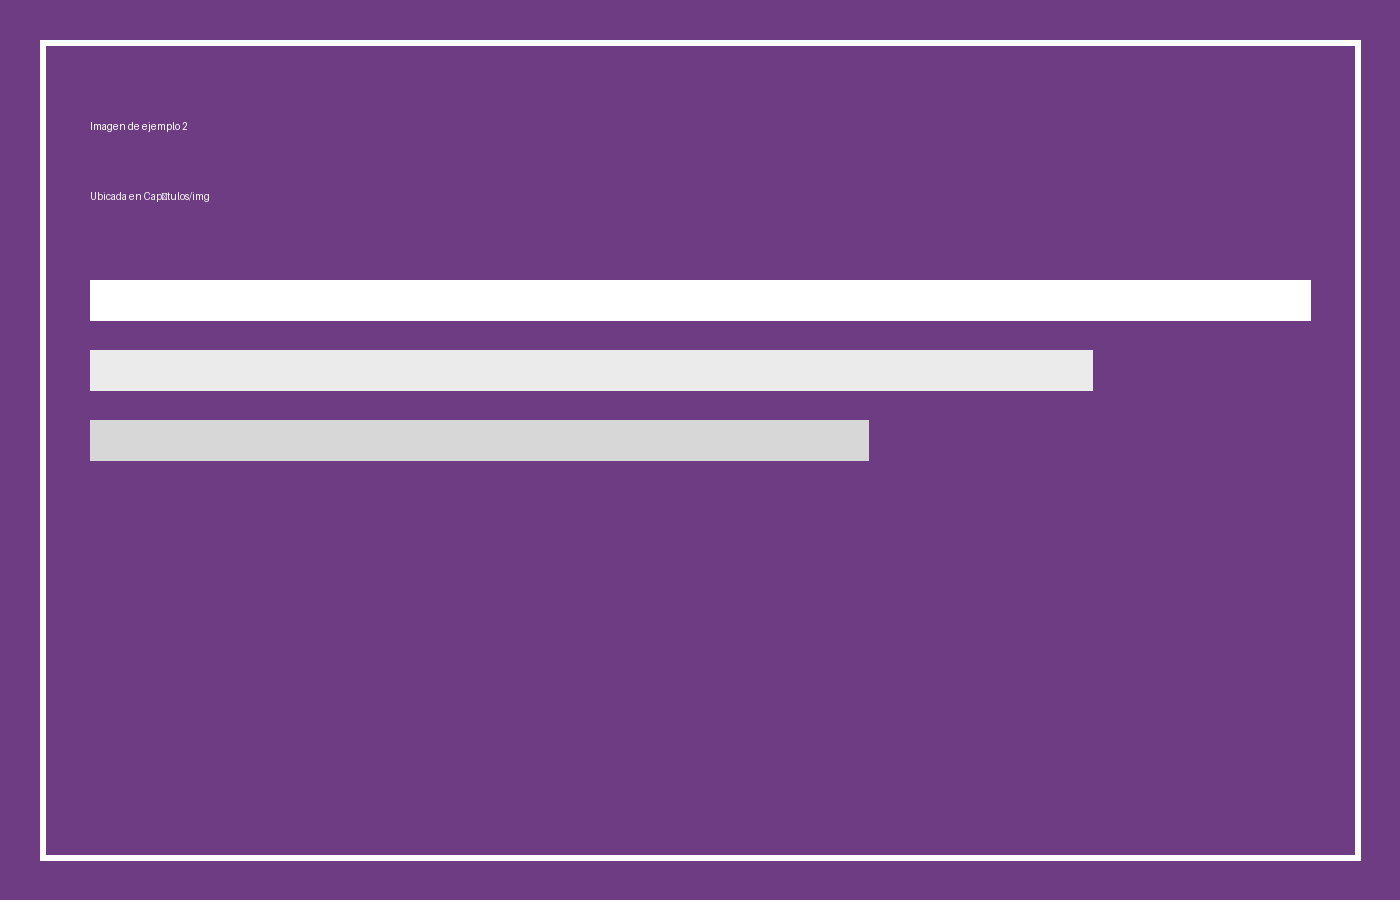
\includegraphics[width=0.80\textwidth]{Capítulos/img/img_ejemplo_2.png}
  \caption{Ejemplo de imagen para evidenciar interfaz, panel o consola de operación.}
  \label{img:ejemplo_2}
\end{imagen}
\elaboradopor{Estudiante}
\fuente{Evidencia del entorno de prueba}

\subsection{Ejemplo de Ecuación 2}
Ejemplo de referencia a ecuación: la Ecuación~\ref{eq:mejora} calcula el porcentaje de mejora de una métrica respecto al valor inicial.

\begin{equation}
\label{eq:mejora}
Mejora\,(\%) = \frac{Valor_{antes} - Valor_{despues}}{Valor_{antes}} \times 100
\end{equation}
\addeqtolist{Cálculo porcentual de mejora obtenida}

\subsection{Ejemplos de Referencias Cruzadas}
Ejemplo 1 de referencia cruzada entre capítulos: el análisis base se desarrolla en el Capítulo~\ref{chap:introduccion}, mientras que el enfoque metodológico se detalla en el Capítulo~\ref{chap:metodologia}.

Ejemplo 2 de referencia cruzada entre elementos: para relacionar diseño y validación se puede enlazar el apartado \emph{\nameref{sec:diseno_solucion}} (Capítulo~\ref{chap:metodologia}) con la Tabla~\ref{tab:ejemplo_2}, la Imagen~\ref{img:ejemplo_1} y la Ecuación~\ref{eq:disponibilidad}.

\section{Cronograma y Presupuesto}
\textit{[Presentar la planificación de las fases de ejecución del proyecto y el detalle de los costos asociados a hardware, licencias, servicios u otros recursos.]}
